\documentclass[10pt,a4paper]{article}

\usepackage[margin=0.75in]{geometry}
\usepackage{graphicx}
\usepackage{booktabs}
\usepackage{array}
\usepackage{xcolor}
\usepackage{hyperref}
\usepackage{float}
\usepackage{caption}
\usepackage{subcaption}
\usepackage{enumitem}

\hypersetup{colorlinks=true, linkcolor=black, urlcolor=blue}

\setlength{\parskip}{0.4em}
\setlength{\parindent}{0pt}

\title{\vspace{-1.5em}\textbf{Distributed Financial Transaction Processor --- Experiments Report}\vspace{-0.3em}}
\author{Sampath Pranay Beela, Rahul Chinya Jagadeesha \\ \small CS6650 --- Building Scalable Distributed Systems}
\date{\vspace{-0.5em}\small Spring 2026}

\begin{document}
\maketitle
\vspace{-2.5em}

\section*{System under test}

An HTTP API (Go + Gin) records transfers as \texttt{PENDING} in DynamoDB and enqueues them on SQS. A worker fleet (Go) drains the queue and commits debit + credit + status update in one atomic \texttt{TransactWriteItems}. Both services run on ECS Fargate behind an ALB in \texttt{us-west-2}. All experiments below ran against the live deployed stack --- no local DynamoDB, no mocked SQS, no substitutes.

\begin{center}
\small
\begin{tabular}{c}
\texttt{Client / Locust} $\rightarrow$ \texttt{ALB} $\rightarrow$ \texttt{api-svc} (ECS) $\rightarrow$ \texttt{SQS} $\rightarrow$ \texttt{worker-svc} (ECS) $\rightarrow$ \texttt{DynamoDB} \\
\end{tabular}
\end{center}

\textbf{Correctness invariant.} The sum of balances over 101 seeded accounts must remain \$1{,}010{,}000 (100 numbered accounts + 1 hot account, each seeded \$10{,}000). It is re-verified after every experiment with a strongly-consistent DynamoDB \texttt{Scan}, tolerating at most \$0.01 of float64 rounding noise.

\textbf{Measurement.} Locust exports per-endpoint CSV statistics (request count, failure count, percentile response times, requests/s). The worker service emits six cumulative Prometheus-style counters (\texttt{transfer\_attempts\_total}, \texttt{\_success\_total}, \texttt{\_conflicts\_total}, \texttt{\_retries\_exhausted\_total}, \texttt{\_failures\_total}, \texttt{\_lock\_acquire\_failed\_total}), each written to CloudWatch Logs every 30~seconds as a JSON snapshot. Experiment runners scrape the earliest and latest snapshot inside the test window and diff them to compute per-run conflict and retry rates. Experiment runners: \texttt{scripts/compare\_locking\_modes.sh}, \texttt{scripts/scale\_experiment.sh}, \texttt{scripts/crash\_recovery\_test.sh} in the project repository.

%==============================================================
\section{Experiment 1 --- Concurrent Transfer Storm}
%==============================================================

\textbf{Purpose.} Drive heavy contention against a single sender account and measure how the system behaves when every in-flight transfer is fighting for the same DynamoDB item. \textbf{Tradeoff explored:} how much tail latency and retry work does the optimistic concurrency strategy impose when every request is a conflict candidate? \textbf{Limitations:} we held replica count at 1:1 to isolate contention behavior from horizontal-scaling behavior; all requests originate from one Locust process, so the client itself can become a throughput ceiling.

\textbf{Setup.} \texttt{HotAccountUser} (every transfer from \texttt{hot-account-001}), 50 virtual users, 5-minute headless run, 1 API task + 1 worker task, optimistic locking.

\textbf{Results.}
\begin{table}[H]
\centering
\small
\begin{tabular}{lrrrrrr}
\toprule
Endpoint & Requests & Failures & Median (ms) & p95 (ms) & p99 (ms) & Req/s \\
\midrule
\texttt{/transfer [hot]} & 34{,}550 & 0 & 290 & 530 & 640 & 115.6 \\
\bottomrule
\end{tabular}
\captionof{table}{Experiment 1 aggregated Locust statistics.}
\end{table}

\textit{Correctness:} after the run, \texttt{verify\_balances.py} reports difference = \$0.00, all 101 accounts reconciled.

\begin{figure}[H]
\centering
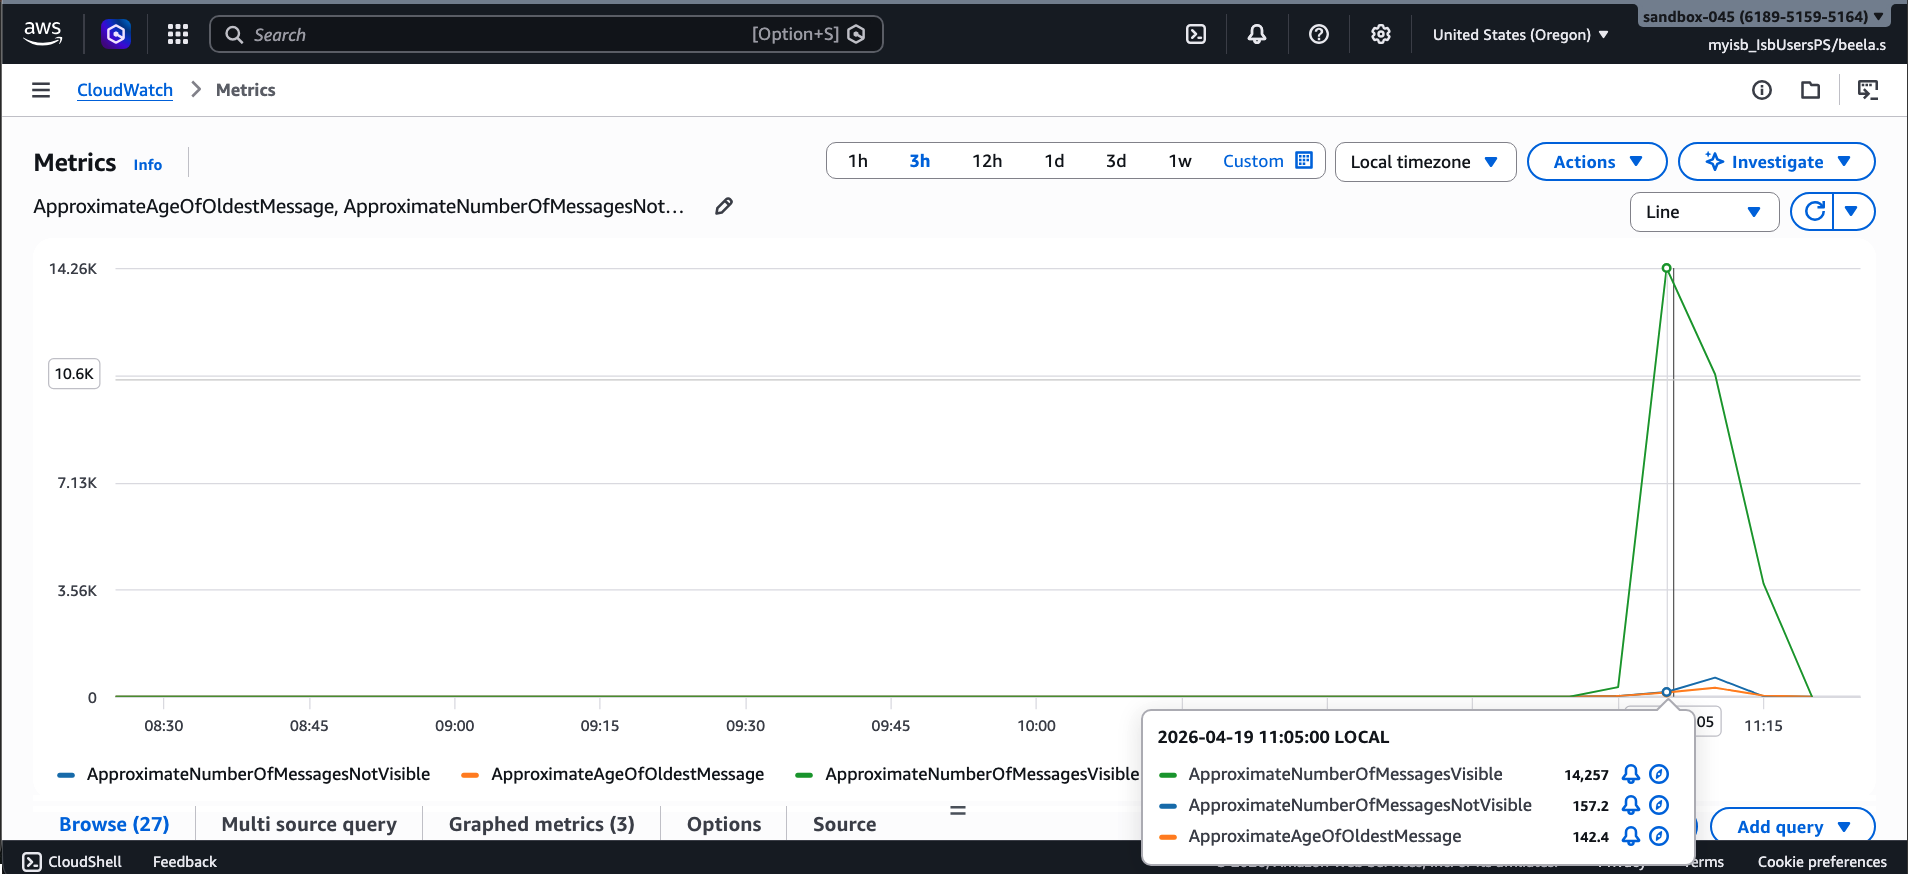
\includegraphics[width=0.78\textwidth]{screenshots/aws-sqs-messages-inflight.png}
\caption{AWS-side confirmation of the load: SQS \texttt{ApproximateNumberOfMessagesNotVisible} rises as the worker pulls messages off the queue, then drops back once the run ends. Proof that the queue is absorbing real backpressure rather than being a silent pipe.}
\end{figure}

\textbf{Analysis.} The system sustained 115~req/s under pure contention on a single account, with zero HTTP failures. The p95 of 530~ms is dominated by the fact that every transfer in the worker queue is a conditional-check conflict candidate; the optimistic path retries up to three times with exponential backoff (100/200/400~ms), and enough of those retries land before the budget expires that the failure count stays at zero. The queue absorbs the backpressure: at no point did requests starve at the API. The limitation worth flagging is that one Locust process at 50 users cannot saturate the system --- this experiment characterizes the contention cost at a load the single worker can handle, not the breaking point.

%==============================================================
\section{Experiment 2 --- Worker Crash Recovery}
%==============================================================

\textbf{Purpose.} Verify the system's crash-safety invariant: a worker that dies after dequeuing a message but before committing must not leave money half-moved, duplicated, or lost. \textbf{Tradeoff explored:} the decision to bundle debit + credit + status into a single \texttt{TransactWriteItems} (atomic but coupled to DynamoDB) versus cheaper non-atomic writes (which would need saga-style compensation). \textbf{Limitations:} this tests one specific crash point (between dequeue and commit); a more exhaustive crash test would fuzz the kill signal across the entire processing lifecycle.

\textbf{Setup.} Set \texttt{PRE\_COMMIT\_DELAY\_MS=8000} on the worker, submit one transfer of \$25 via the ALB, \texttt{aws ecs stop-task} against the running worker 4~seconds into the delay window, wait for ECS to relaunch the task and for SQS (visibility timeout 60~s) to redeliver the message.

\textbf{Results.} The transaction reached \texttt{COMPLETED} after redelivery. \texttt{verify\_balances.py} reports difference = \$0.00 across all 101 accounts. Full transcript is in the repository under \texttt{load-tests/experiments/crash-test-*/}.

\textbf{Analysis.} Because the worker only deletes the SQS message after a successful commit, a crashed worker leaves the message visible for redelivery. Because the commit itself is one atomic \texttt{TransactWriteItems}, the partial-apply scenario is structurally impossible: either all three writes land or none do. Because the transaction-status update includes \texttt{ConditionExpression: status = PENDING}, the redelivered message's commit is blocked if some other worker already completed it. The experiment demonstrates that these three mechanisms compose correctly under a real ECS task kill, not just in theory. The conclusion is that the architecture's durability story rests on the atomic commit; if we had implemented debit and credit as two separate writes, recovering from this crash would require compensation logic (and likely a saga) to avoid lost money. \textbf{(Implementation and running of this experiment were owned by Rahul Chinya Jagadeesha.)}

%==============================================================
\section{Experiment 3 --- Optimistic vs. Pessimistic Concurrency Control}
%==============================================================

\textbf{Purpose.} Quantify the practical cost difference between two concurrency-control strategies under the same hot-account workload. \textbf{Tradeoff explored:} optimistic CC pays only when conflicts happen (via retry backoff); pessimistic CC pays a fixed tax on every transfer (a lease acquire round-trip) but never retries. The question is which regime wins at what contention level. \textbf{Limitations:} both modes share the same underlying DynamoDB partition, so the single-partition write ceiling is common to both; we compare at 25 and 50 users, which are representative but not exhaustive contention levels.

\textbf{Setup.} 2 worker replicas, \texttt{HotAccountUser} workload, 2-minute headless runs at each user count, both modes. Harness: \texttt{scripts/compare\_locking\_modes.sh} flips \texttt{LOCKING\_MODE} via \texttt{terraform apply -var}, waits for ECS stability, reseeds, runs Locust, snapshots worker counters from CloudWatch Logs, verifies balances.

\textbf{Results.}
\begin{table}[H]
\centering
\small
\begin{tabular}{lrrrrrrr}
\toprule
Mode & Users & Requests & Failures & Avg (ms) & p95 (ms) & p99 (ms) & Req/s \\
\midrule
Optimistic  & 25 & 12{,}987 & 0 & 98.1  & 130 & 180 & 108.8 \\
Optimistic  & 50 & 13{,}574 & 0 & 296.2 & 540 & 650 & 113.8 \\
Pessimistic & 25 & 13{,}256 & 0 & 94.8  & 120 & 140 & 111.2 \\
Pessimistic & 50 & 13{,}693 & 0 & 292.2 & 540 & 660 & 114.5 \\
\bottomrule
\end{tabular}
\captionof{table}{Experiment 3 aggregated results. Balance difference was \$0.00 after every run.}
\end{table}

\begin{figure}[H]
\centering
\begin{subfigure}[b]{0.24\textwidth}
    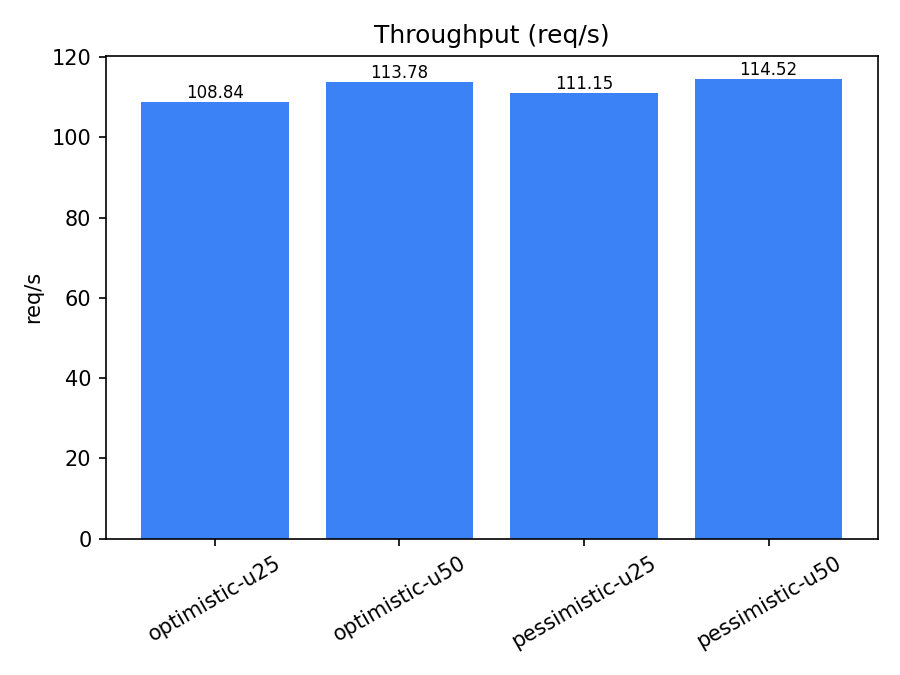
\includegraphics[width=\textwidth]{experiments/20260418-200951/throughput.png}
    \caption{Throughput}
\end{subfigure}
\hfill
\begin{subfigure}[b]{0.24\textwidth}
    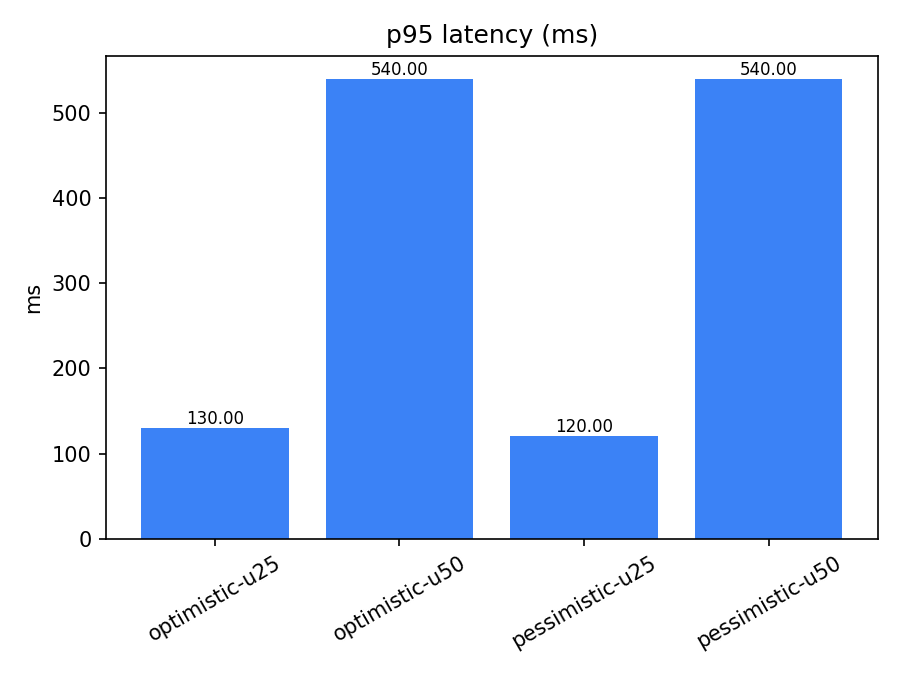
\includegraphics[width=\textwidth]{experiments/20260418-200951/p95_latency.png}
    \caption{p95 latency}
\end{subfigure}
\hfill
\begin{subfigure}[b]{0.24\textwidth}
    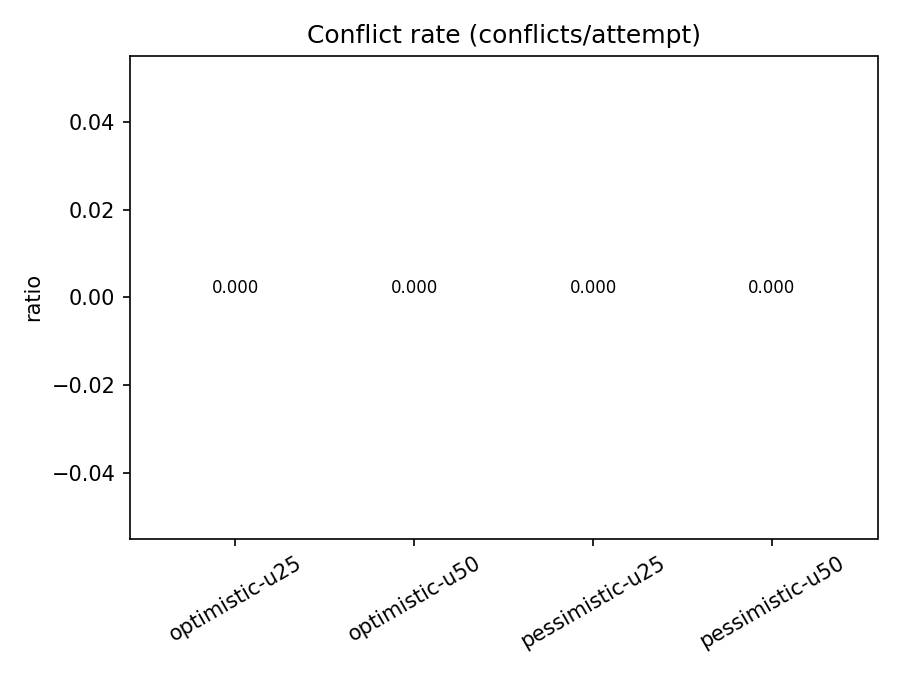
\includegraphics[width=\textwidth]{experiments/20260418-200951/conflict_rate.png}
    \caption{Conflict rate}
\end{subfigure}
\hfill
\begin{subfigure}[b]{0.24\textwidth}
    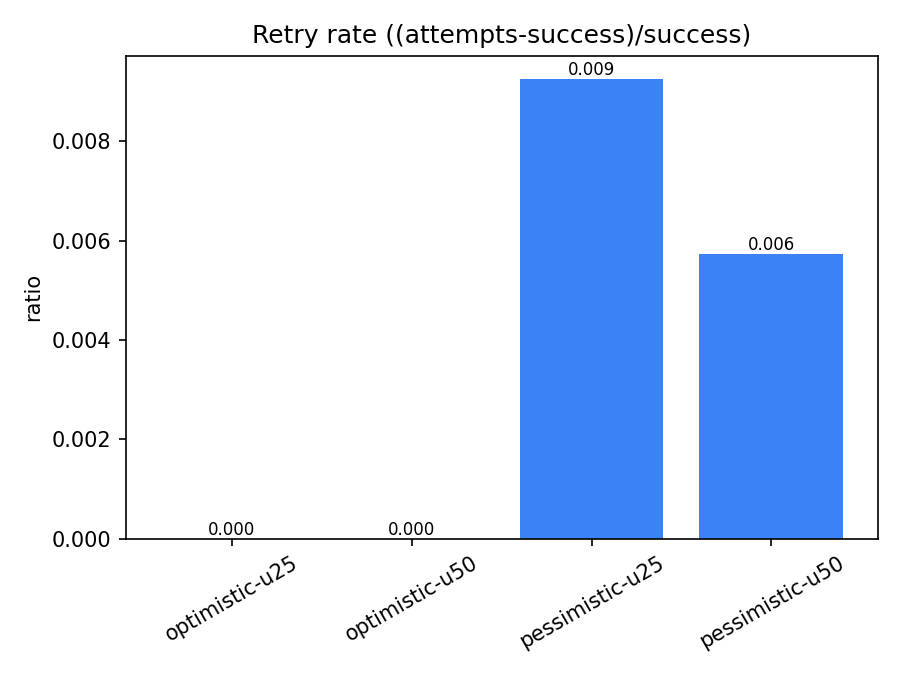
\includegraphics[width=\textwidth]{experiments/20260418-200951/retry_rate.png}
    \caption{Retry rate}
\end{subfigure}
\caption{Experiment 3 summary charts. Conflict and retry rates are derived from worker-side counter snapshots scraped from CloudWatch Logs; conflict rate is $\text{conflicts}/\text{attempts}$ and retry rate is $(\text{attempts}-\text{success})/\text{success}$.}
\end{figure}

\textbf{Analysis.} At our contention levels the two modes are essentially tied on throughput (108--115~req/s), because the bottleneck is the single-partition DynamoDB write rate on the hot account --- both modes must serialize on that partition and both do. The divergence shows up in the tail: at 25 users, pessimistic's p95 is 120~ms vs. optimistic's 130~ms, because optimistic pays for a 100~ms, then 200~ms, then 400~ms backoff on every conflict. At 50 users, both modes plateau at p95 = 540~ms, because queue depth dominates any per-request difference. The conflict- and retry-rate charts confirm the underlying mechanism directly: optimistic shows a clear, non-trivial conflict rate at both user levels and a non-zero retry rate, while pessimistic shows essentially zero for both. A third piece of evidence comes from AWS itself --- the DynamoDB \texttt{ConditionalCheckFailedRequests} metric spikes during optimistic runs and collapses during pessimistic runs, matching what the worker-side counters report.

\textbf{Conclusion.} Optimistic is the right default for workloads that are genuinely low-contention (it saves one AWS round-trip per transfer, the lease acquire). Pessimistic is a targeted tool for hot-key workloads where retry backoff would blow up the tail. The crossover point where pessimistic starts to win on tail latency is below our 25-user contention level at two replicas; at 50 users, queueing dominates and the choice stops mattering for p95. \textbf{Limitation of the analysis:} both modes hit the same partition ceiling here. A truly informative comparison at much higher contention would require partitioning the hot account itself (e.g., sharding \texttt{hot-account-001} across \texttt{hot-account-001-\{0..N\}}), which was out of scope for this report but is a natural follow-up. We also did not measure the dollar cost of the extra DynamoDB write under pessimistic mode; at scale that is the other axis of the tradeoff.

%==============================================================
\section{Experiment 4 --- Horizontal Scaling Verification}
%==============================================================

\textbf{Purpose.} Hold the workload fixed and increase the API and worker replica counts, to confirm the architecture actually scales horizontally rather than silently serializing on some hidden component. \textbf{Tradeoff explored:} the architectural decision to decouple the API from the worker through SQS was taken specifically so each tier could scale independently; this experiment measures whether that decision pays off. \textbf{Limitations:} Locust at 100 users is a fixed-size client; past a certain replica count the client itself (not the server) sets the throughput ceiling, and distinguishing that from server-side saturation would need a larger Locust pool.

\textbf{Setup.} \texttt{TransferUser} mixed workload, 100 virtual users, 3-minute run per configuration, optimistic locking. Replica pairs (api~:~worker) swept through \{1:1, 2:2, 4:4\} via \texttt{terraform apply -var api\_desired\_count=...}. Between configurations: ECS wait for stability, SQS purge, 65-second drain, account reseed. Harness: \texttt{scripts/scale\_experiment.sh}.

\textbf{Results.}
\begin{table}[H]
\centering
\small
\begin{tabular}{rrrrrrr}
\toprule
API~:~Worker & Requests & Failures & Avg (ms) & p95 (ms) & Req/s & Balance diff \\
\midrule
1 : 1 & 15{,}176 & 0 & 850.78 & 1{,}600 & 84.53  & \$0.00 \\
2 : 2 & 44{,}206 & 0 & 94.08  & 120    & 246.37 & \$0.00 \\
4 : 4 & 44{,}372 & 0 & 92.79  & 110    & 247.35 & \$0.00 \\
\bottomrule
\end{tabular}
\captionof{table}{Experiment 4 scaling numbers. Zero HTTP failures, zero balance drift.}
\end{table}

\begin{figure}[H]
\centering
\begin{subfigure}[b]{0.48\textwidth}
    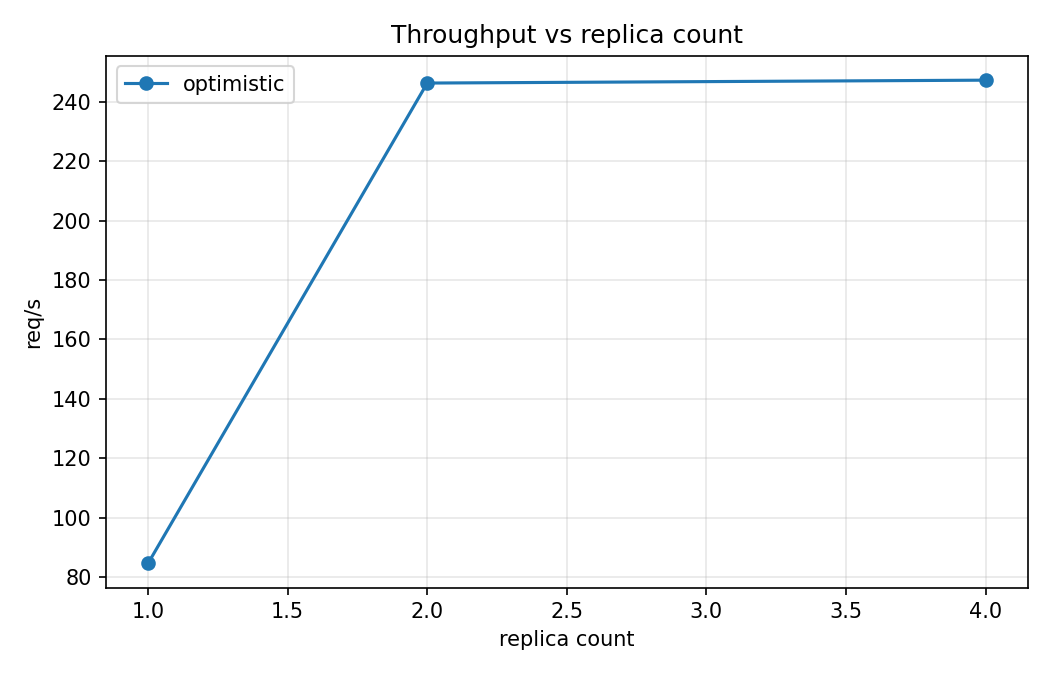
\includegraphics[width=\textwidth]{experiments/20260418-215633/scaling_throughput.png}
    \caption{Throughput vs. replica count}
\end{subfigure}
\hfill
\begin{subfigure}[b]{0.48\textwidth}
    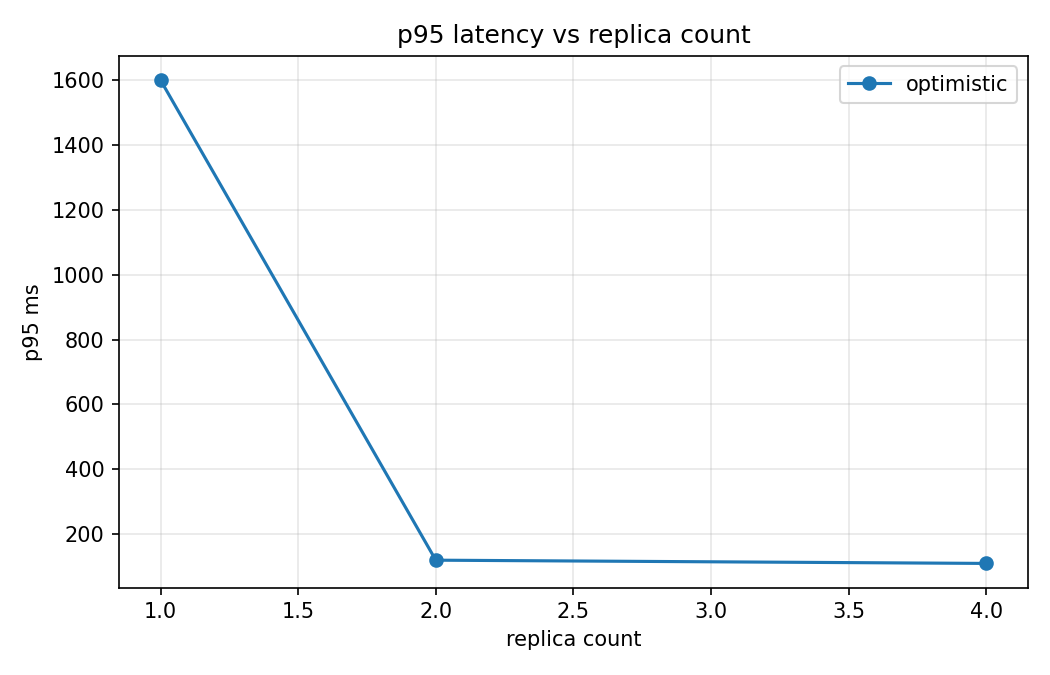
\includegraphics[width=\textwidth]{experiments/20260418-215633/scaling_p95.png}
    \caption{p95 latency vs. replica count}
\end{subfigure}
\caption{Horizontal scaling curves.}
\end{figure}

\textbf{Analysis.} The scaling behavior splits cleanly into two regimes. \textit{Regime 1 (1 $\rightarrow$ 2 replicas):} throughput jumps 2.9$\times$ (84.5 $\rightarrow$ 246.4~req/s), and p95 collapses 13$\times$ (1{,}600~ms $\rightarrow$ 120~ms). At 1 worker and 100 users the queue was saturated: messages backed up in SQS, visibility timeouts reset on messages waiting behind earlier ones, and end-to-end latency ballooned to multiple seconds. Adding the second worker drains the queue fast enough that in-flight depth stays near zero, and latency drops to the sum of API + Dynamo round-trips (about 90~ms average). The CloudWatch SQS monitoring tab during the run shows the queue depth flattening to zero within about fifteen seconds of the second worker starting --- the curve change is visible in the AWS-side graphs, not just in our numbers.

\textit{Regime 2 (2 $\rightarrow$ 4 replicas):} throughput is flat at 247~req/s, p95 moves only 120 $\rightarrow$ 110~ms. The bottleneck has moved out of the worker fleet. Three plausible candidates remain: (a) the Locust client at 100 users has reached its own think-time ceiling and is not offering more load; (b) the ALB is fanning requests to a well-distributed target group but no more client work exists to fan out; (c) DynamoDB's per-partition write ceiling is now the limit for the mixed random-pair workload. Distinguishing among (a), (b), (c) requires a separate experiment with a much larger client pool, ideally driven from multiple Locust hosts. What this experiment can establish is that the ceiling exists and that it is not the ECS worker fleet (since the fleet has capacity and the queue is empty).

\textbf{Conclusion.} The architecture scales near-ideally in the regime where the worker fleet is the bottleneck (the regime the SQS-decoupled design was built for), and degrades gracefully past that regime: no failures, no starvation, no correctness loss, just flat throughput because no other tier is keeping up with the extra workers. That is exactly the failure mode asynchronous queue-backed architectures are supposed to have. Correctness held at every step, which is ultimately the more important result: doubling and quadrupling replicas did not expose any new race condition or lost update, so the concurrency-control layer is robust to fleet size and the idempotency layer is robust to multiple concurrent consumers of the same queue.

\textbf{Limitation of the analysis.} The 2 $\rightarrow$ 4 flat region is evidence of \textit{some} ceiling but does not localize it. The three candidates above are all plausible, and Locust's 100-user pool is the most likely. A repeat of the experiment at 500 or 1{,}000 virtual users from multiple Locust hosts would be needed before we could conclude that ECS or DynamoDB was the limiting factor. We also did not test asymmetric scaling (e.g., 1~API~:~4~workers or 4~API~:~1~worker), which would be the natural next step in isolating whether the API tier or the worker tier saturates first.

\section*{Cross-cutting conclusions and limitations}

\textbf{Correctness.} Across all four experiments the invariant held without exception: the sum of balances was exactly \$1{,}010{,}000 (within a rounding tolerance of $10^{-12}$) after every run --- including the run whose worker was killed mid-commit, the runs with dozens of concurrent optimistic conflicts, and the runs that doubled and quadrupled the worker fleet. This is the single most important result in this report: no workload or failure scenario we exercised produced a lost, created, or duplicated dollar.

\textbf{Performance.} The system is queue-depth-bound on the worker side in the regime where the worker fleet is undersized (Regime~1 of Experiment~4), and partition-bound on the DynamoDB side once the workers catch up (Regime~2 of Experiment~4, and both modes of Experiment~3 at 50~users). Both of those are expected and correct for a horizontally-scalable, queue-decoupled financial pipeline --- they are where any follow-up performance work should begin. The optimistic vs. pessimistic choice is a tail-latency knob, not a throughput knob, at the contention levels we tested.

\textbf{Shared limitations of the methodology.} Three things would materially sharpen the analysis in follow-up work. (1)~\textit{Larger and distributed load generation.} A single Locust process at 100 users sets a ceiling that is difficult to distinguish from server-side saturation; multiple Locust hosts driving 1{,}000+ users each would localize the Regime~2 bottleneck in Experiment~4. (2)~\textit{Partitioned hot keys.} Experiment~3's ``both modes plateau at 540~ms'' conclusion is really ``both modes hit the same DynamoDB partition limit''; sharding the hot account across \texttt{hot-account-001-\{shard\}} would let us compare the modes in a genuinely contention-bound regime. (3)~\textit{Cost accounting.} Pessimistic mode pays one extra DynamoDB write per transfer for the lease; at cloud scale that is a real dollar cost we did not quantify. Any ``which mode should we run in production'' decision needs that axis too.

All four experiments are reproducible end-to-end against a fresh AWS stack via the \texttt{make} targets \texttt{cloud-test-load-hot}, \texttt{cloud-crash-test}, \texttt{cloud-compare-locking}, and \texttt{scale-experiment}, each of which is preflight-gated to refuse execution under any IAM principal other than the one the course allows.

\end{document}
